%!TEX root = series of tubes.tex
\section{Discussion}

The promise of 3D printing is two-fold: it enables the manufacturing of complex objects at low volumes, and it allows for the manufacturing of geometries that are impossible to create using traditional techniques like injection molding.  Printing pipes to prototype interactive objects exploit both advantages. Prototypes by definition are low-volume parts, and pipes require complex interior geometries that are very difficult or impossible to produce using other processes. Our work has focused on routing pipes that are then later manually filled after a print has completed. However, the fundamental operations of 3D path routing and topology specification that our tool offers will remain relevant as 3D printing technology advances. Multi-material printers are already available; as they advance and support the embedding of additional materials (e.g., conductive), \systemname can enable designers to efficiently specify where different functional materials should be placed at design time.

We described a design space and fabricated example objects to demonstrate some of the interactions that can be aided by pipe routing. There are many additional possibilities for leveraging sensing and actuation techniques from the HCI literature and extending their use in 3D-printed objects. We briefly survey some of them.

\subsection{Inputs and Outputs}

Pipe-based outputs can address the five senses: visual, aural, haptic, and olfactory/gustatory.  As we have already discussed many input techniques through our example objects, we focus our discussion around output.  %In addition to outputs we mention explicitly, any outputs possible using traditional electronic components are possible using conductive material in pipes.

\begin{figure}[h]
\centering
    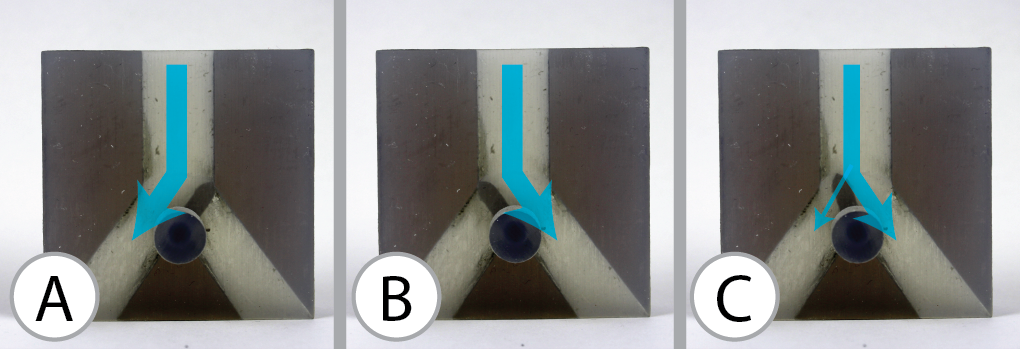
\includegraphics[width=3.4in]{figures/gates.png}
\caption{By attaching a servo to a gate structure, it is possible to direct fluid through that pipe.  The gate not only has binary positions (a) and (b), but can direct fractional flow, as well (c).  This could be used, for example, in science exhibits.}
\label{fig:direct}
\end{figure}

\emph{Visual} outputs can be mediated by gases, liquids, solid, particulates, or threadables.  Pneumatic actuation (as in PneUIs \cite{Yao-pneui} or Harrison's latex buttons \cite{Harrison-buttons}) can provides shape-changing interfaces if maelleable materials can be printed. 
%Gases carrying smoke also offer visual feedback. 
Air bubbles in liquids can also convey information~\cite{Heiner1999Percolator}. Splitting and mixing of colored liquids can be used as a display tactic; liquids can also be mixed in specific concentrations by servo-controlled gate structures as in Figure \ref{fig:direct}. %additionally mechanical motion can be fluid-mediated. 

\emph{Aural} outputs can be created with gases.  Pipes and cavities can act as resonators can be leveraged to create 3D-printed sound chambers with explicitly designed sound characteristics~\cite{Zoran-flute} (see Figure \ref{fig:ocarina}).  %All that is necessary for this is an enclosed chamber with a pipe connected to it via a narrow neck-point (see Figure \ref{fig:ocarina}).  
Passive sound amplification and sound redirection are also possible using pipes, and sensing of some interactions, e.g., \emph{tapping and grasping}, can be sensed acoustically.  Due to differential sound conductivity in different printed materials, solid pipes of a material with greater conductivity (i.e., rigid, high-density) can be embedded in a model of a lesser conductivity (i.e., softer).  A microphone or piezo placed at the system-side of these sound-conducting pipes can determine where the model was tapped and how it was tapped.  Active acoustic sensing as described in Touch \& Activate \cite{Ono-touchandactivate} is also possible; this technique would allow for particular areas of interest (connected to rigid pipes) to be touch sensitive and enable grasp sensing.

\begin{figure}[h]
\centering
    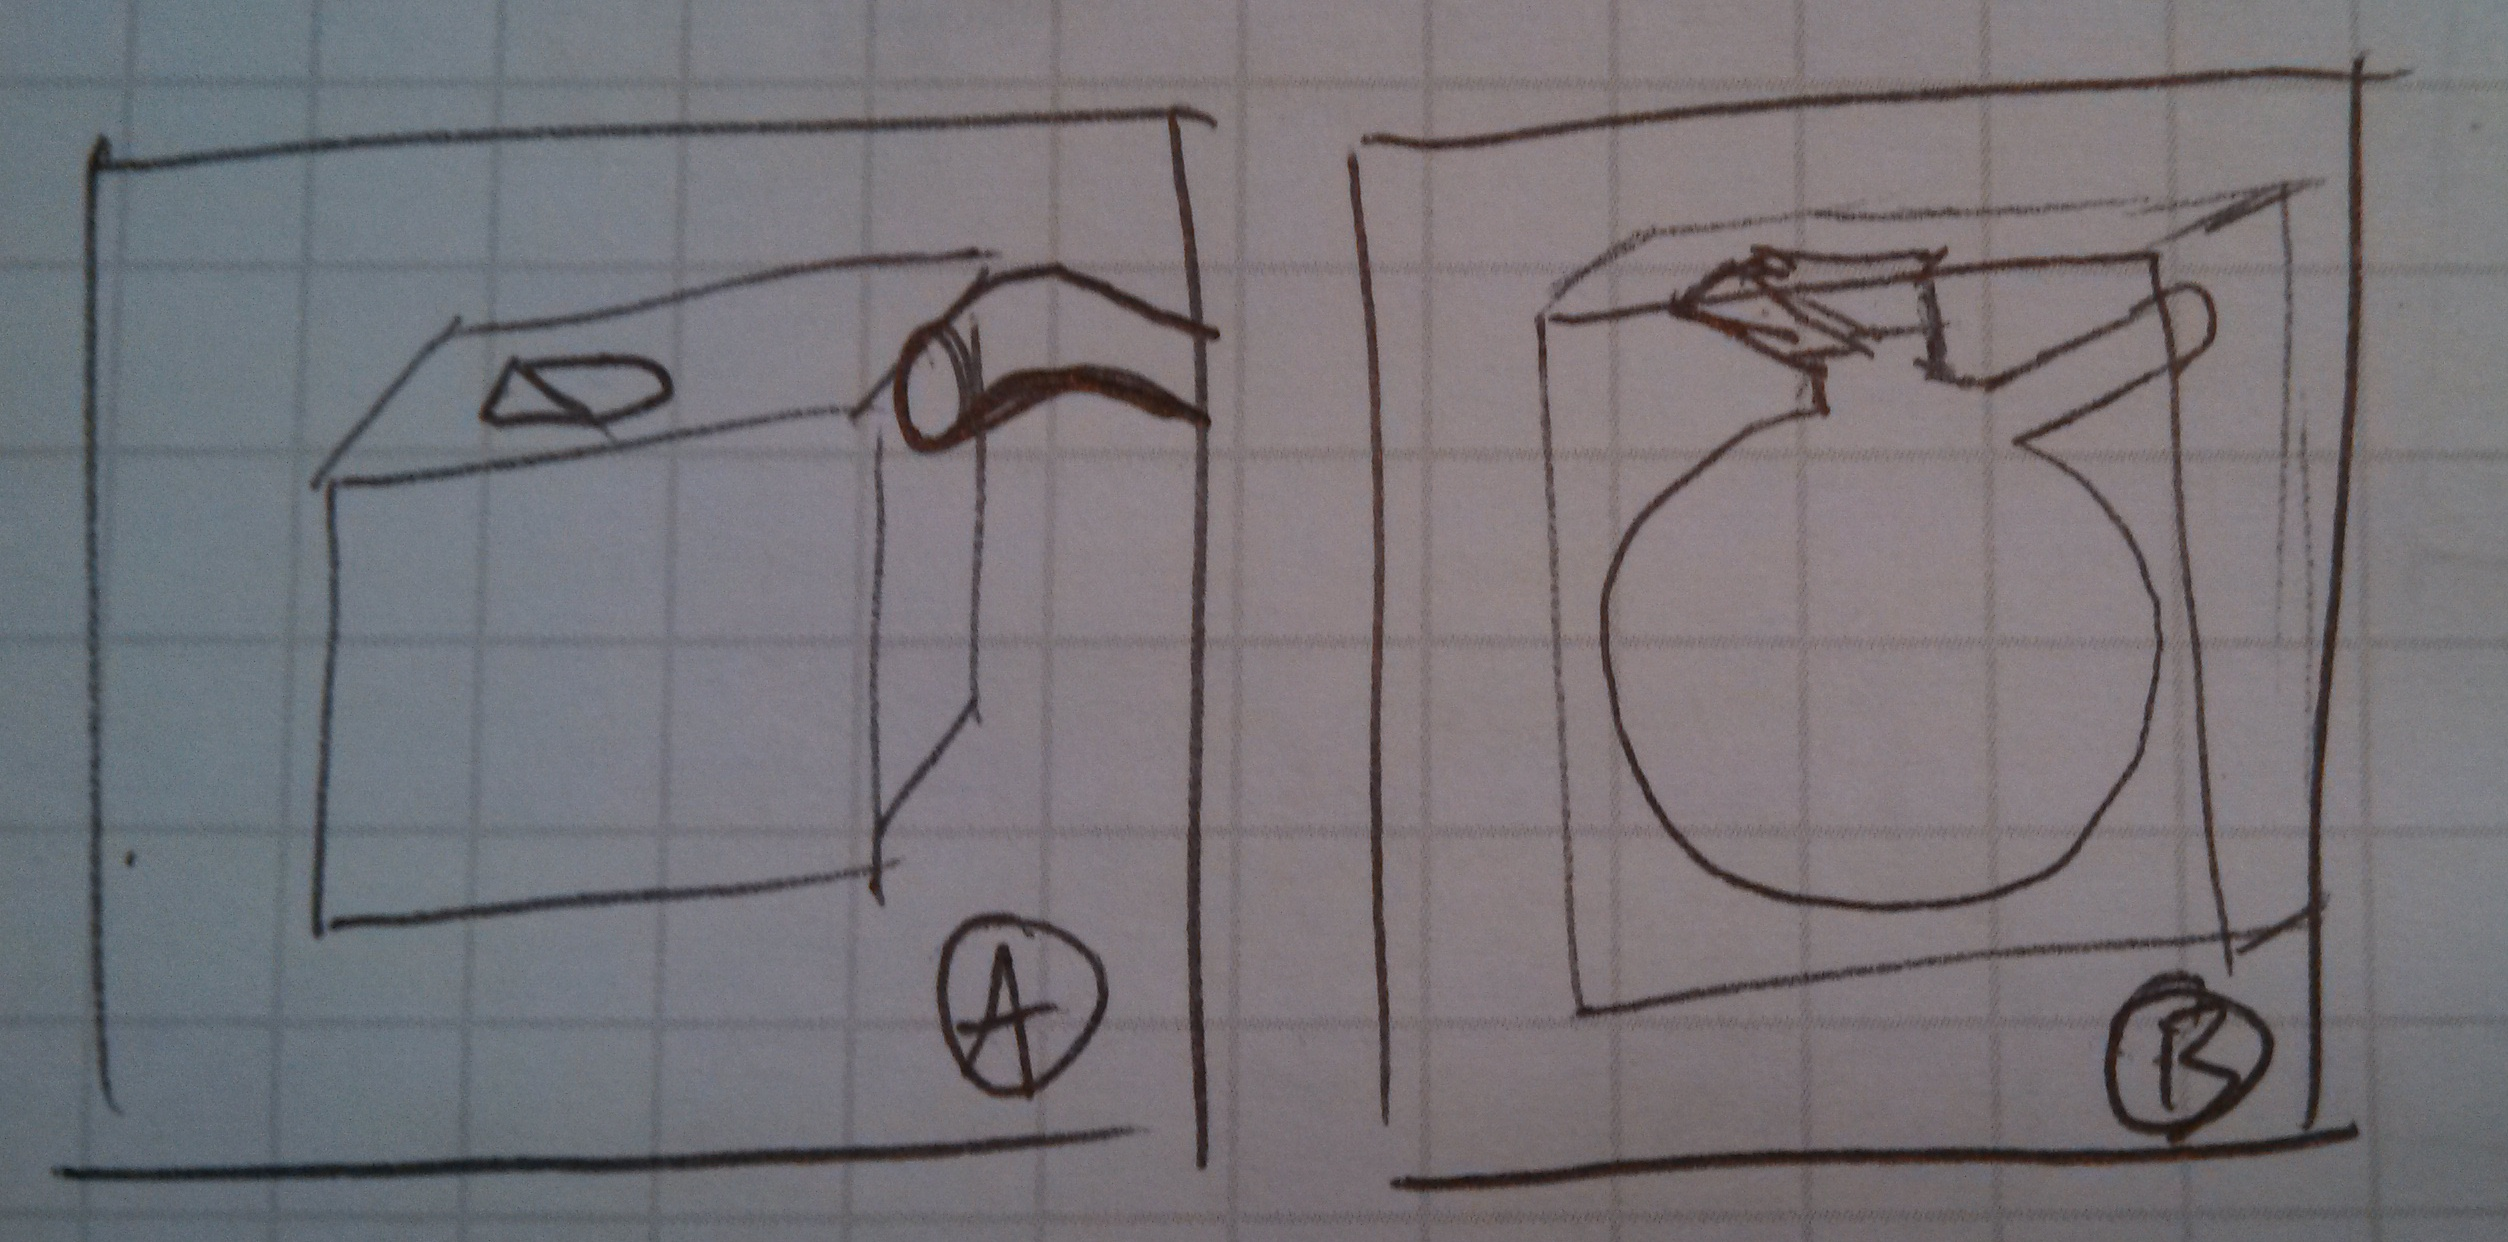
\includegraphics[width=3.4in]{figures/placeholder/helmholz.jpg}
\caption{Some possible pipe uses.  The printed whistle in (a) is a Helmholz resonator: it creates a sound when air is blown through the pipe at the front, because air compresses at the small neck joint between the internal chamber and the pipe.  In (b), a capacitor manufactured on a 3D printer coated post-print with copper paint.  This particular one holds a charge of \valkyrie{XX}.  (c) gives a comparison of pipe-based resistors, also filled with copper paint.  For a cylindrical wire, resistance = $\rho\frac{l}{\pi r^2}$, where $\rho$ is based on the conductivity of the medium.  In our case, because $r << l$, $resistance(B) < resistance(C) < resistance(A)$.}
\label{fig:ocarina}
\end{figure}


\emph{Haptic} outputs are possible through compressible and incompressible fluids, as discussed, or through threadable inputs: e.g., muscle wire can be inserted in flexible pipes and actuated, similar to shape changing interfaces \cite{Coelho-shapechanging}.

\emph{Olfactory} and \emph{gustatory} outputs can be created through the mixing and splitting of pipes carrying scented or flavored fluids, respectively~\cite{kaye2004making}.

\subsection{Identification}
In addition to active inputs from users, pipes can be used for passive \emph{identification}.  Fully-enclosed pipes which are not visually apparent can change the weight, acoustic resonance, or capacitive signature of a 3D object. 

Each of these properties could be used for object identification. As seen in Touch \& Activate \cite{Ono-touchandactivate}, different objects have different acoustic signatures.  As such, two objects that are visually identical but have differing internal chamber geometry on their interior may be distinguished acoustically.  Thus we can recall an object's identity once its acoustic signature has been recorded.  Similarly, the Touch\'{e} system \cite{Sato-touche} relies on distinguishing \emph{capacitive} signatures of objects, both in static states and as their boundary conditions are changed by human interaction. Weight could also be used as a simple metric of object identity, but would be less distinctive than acoustic or capacitive signatures.

%We have experimented with intentional encoding.  Semi-closed pipes can function as resonance chambers.  A pipe's resonant frequency can be measured by attaching a speaker and microphone to it, sweeping frequencies with the speaker, and performing a Fourier transform on the resultant signal from the microphone.  Peaks in the transformed data correspond to resonant frequencies of the object.  Intentional encoding in the case of capacitance is significantly more difficult, and we leave it to future work.  Encoding of weight is trivial by creating fully-enclosed chambers inside an object.  This is similar to Infrastructs \cite{Willis-infrastructs}.  While their technique requires access a terahertz imaging tool, audio resonance identity encoding requires only a microphone and a speaker.

\subsection{Passive Components}

Printing or injecting conductive material can also be used to design passive components with particular electrical properties. For example, we printed a proof-of-concept  capacitor which features a thin printed plate with hollow cones on either side (see Figure \ref{fig:electronics}A).  After printing, we coated the inner surfaces of capacitor with copper paint.  It now can hold a charge of xx.  Similarly, tubes can be used to create \emph{resistors} in ``printed'' circuitry: a longer or thinner tube has a greater resistance than a shorter or wider one (see Figure \ref{fig:electronics}B).  Internal \emph{antenna} design is also possible, which could lead to new flexibility in, e.g., cell phone design (see Figure \ref{fig:electronics}C). Future design tools could help designers achieve desired electrical properties automatically.
